\section{Pianificazione} \label{section:pianificazione}

Considerate le scadenze indicate in \hyperref[subsection:intro_scadenze]{1.5 Scadenze}, si è deciso di organizzare lo sviluppo del progetto nei seguenti periodi:
\begin{itemize}
  \item \textbf{Analisi preliminare};
  \item \textbf{Progettazione Technology Baseline};
  \item \textbf{Codifica Proof of Concept\glo{}};
  \item \textbf{Progettazione di dettaglio e codifica dei requisiti};
  \item \textbf{Validazione e collaudo}.
\end{itemize}
Per una maggiore comprensione, la suddivisione dei periodi lungo la linea temporale viene riassunta graficamente tramite la seguente sequenza temporale:
\begin{figure}[H]
  \centering
  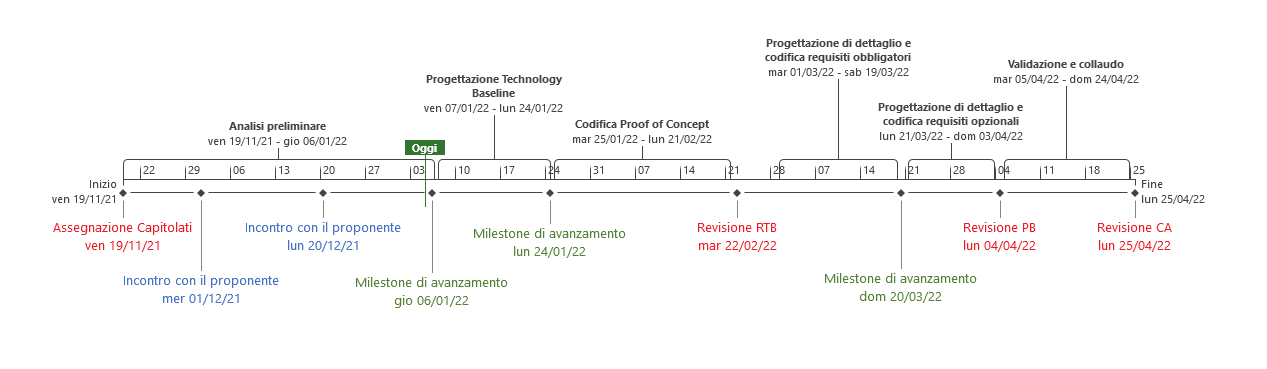
\includegraphics[scale=0.6]{immagini/sequenza_temporale.png}
  \caption{Panoramica della sequenza temporale}
\end{figure}
Il periodo di sviluppo del prodotto è suddiviso in periodi incrementali prefissati. Ogni periodo viene suddiviso in attività, le quali possono essere a loro volta scomposte in sotto-attività più dettagliate.
Le scadenze temporali di alcuni incrementi sono state scelte in base alle revisioni di avanzamento, in modo che il sistema possa evolvere in base ai feedback ricevuti.
Per rappresentare temporalmente le attività viene utilizzato un diagramma di Gantt\glo{}.
\\Le attività possono essere dei seguenti tipi:
\begin{itemize}
  \item \textbf{Attività critiche:} Attività particolarmente importanti per il corretto sviluppo del progetto. La loro data di fine non può slittare e il ritardo di una di esse
        incide gravemente sulle altre, causando ritardi a cascata. Sono indicate con il colore rosso;
  \item \textbf{Attività non critiche:} Attività di minore importanza dalle quali non dipende lo sviluppo generale del progetto. La loro data di fine può essere slittata e non causerebbe ritardi a cascata.
        Sono indicate con il colore blu;
  \item \textbf{Attività di verifica:} Attività poste alla fine dei vari periodi per garantire un controllo sulle altre attività svolte.
        Sono indicate con il colore verde;
  \item \textbf{Evento prefissato:} Rappresenta un particolare evento di durata pari a zero giorni. Può rappresentare una milestone\glo{} interna (rombo di colore verde), la consegna dei documenti
        per una revisione, una revisione di avanzamento (rombo di colore rosso) oppure un incontro con il
        proponente (rombo di colore blu). Sono indicate con un rombo colorato.
\end{itemize}
%%%%%%%%%%%%%%%%%%%%%%%%%%%%%%%%%%%%%%%%%%%%%%%%%%%%%%%%%%%%%%

\subsection{Analisi preliminare} \label{subsection:pianificazione_Analisi}
\textbf{Periodo:} dal 2021/11/19 al 2022/01/06.
\bigskip
\\Questo periodo ha inizio con l'assegnazione del capitolato d'appalto e termina con l'inizio del periodo di Progettazione per la Technology Baseline\glo{}.
Inizialmente vengono individuati sia gli strumenti per il lavoro collaborativo sia quelli più adatti a redigere la documentazione.
Si procede poi con un'analisi preliminare atta ad individuare i requisiti per lo sviluppo del prodotto.
\\Durante questo periodo, a causa dell'inesperienza del gruppo riguardo alle tematiche trattate, si è scelto di dedicare tempo all'autoformazione.
Inoltre vengono redatti ulteriori documenti relativi alle strategie e alla qualità che il gruppo \groupName{} si prefigge di rispettare.
\\Le attività durante questo periodo sono quindi le seguenti:
\begin{itemize}
  \item \textbf{Autoformazione:} Tramite il corso sulla Blockchain\glo{} rilasciato dall'Università di Verona;
  \item \textbf{Norme di progetto:} Vengono subito individuati gli strumenti che saranno utilizzati per la stesura dei documenti e per la collaborazione.
        Le norme sono emanate dall'\roleAdministratorLow{} e il rispetto di quest'ultime dovrà essere certificato dai \textit{verificatori}. Vengono redatte le \docNameNdP{};
  \item \textbf{Piano di progetto:} Basandosi sulle date decise di comune accordo per le revisioni di avanzamento e le scadenze che il gruppo si è prefissato, il \roleProjectManager{} redige il \docNamePdP{}.
        Questa attività risulta essere critica poiché ne deriva l'organizzazione dell'intero gruppo;
  \item \textbf{Analisi dei requisiti:} Tramite il capitolato d'appalto e gli incontri con il proponente, l'\roleAnalystLow{} identifica i requisiti del sistema e redige una prima versione dell'\docNameAdR{}.
        I requisiti evolveranno nel periodo successivo in base ai feedback ricevuti dal proponente;
  \item \textbf{Piano di qualifica:} L'\roleAdministratorLow{} redige i piani e le procedure di gestione per la qualità, mentre il \roleVerifierLow{} illustra l'esito e la completezza delle verifiche. Viene redatto il \docNamePdQ{};
  \item \textbf{Glossario:} Viene creato il \docNameGlo{}. Questo documento viene aggiornato in modo continuativo dai \textit{verificatori} dei documenti aggiungendo termini che necessitano di spiegazione;
\end{itemize}
In questo periodo i ruoli coinvolti sono: \roleProjectManagerLow{}, \roleAdministratorLow{}, \roleAnalystLow{} e \roleVerifierLow{}.

%%%%%%%%%%%%%%%%%%%%%%%%%%%%%%%%%%%%%%%%%%%%%%%%%%%%%%%%%%%%%%

\begin{figure}[H]
  \centering
  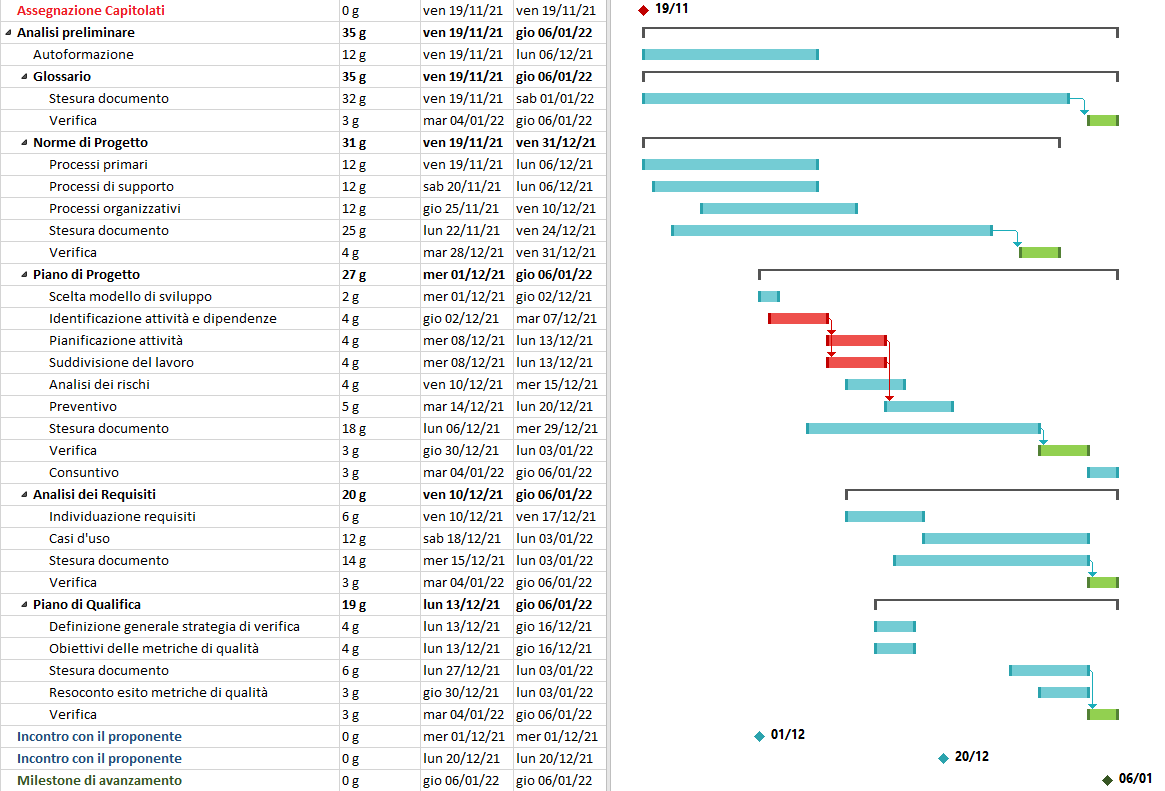
\includegraphics[scale=0.58]{immagini/analisi_preliminare.png}
  \caption{Diagramma di Gantt - Analisi preliminare}
\end{figure}
\pagebreak
%%%%%%%%%%%%%%%%%%%%%%%%%%%%%%%%%%%%%%%%%%%%%%%%%%%%%%%%%%%%%%

\subsection{Progettazione Technology Baseline} \label{subsection:pianificazione_TB}
\textbf{Periodo:} dal 2022/01/07 al 2022/01/24.
\bigskip
\\Questo periodo ha inizio dopo l'Analisi preliminare e finisce con l'inizio della Codifica del Proof of Concept\glo{}.
In corrispondenza del termine di questo periodo verrà fissato un incontro con il proponente in cui verrà presentata la soluzione generale individuata e in cui verranno annotate eventuali correzioni.
Verranno inoltre apportati incrementi ai documenti prodotti nei periodi precedenti.
L'analisi del sistema che viene effettuata in questo periodo serve come base tecnologica e progettuale per la codifica finale del Proof of Concept\glo{}, realizzato nel periodo successivo.
Durante questo periodo vengono effettuati 2 incrementi e 4 modifiche incrementali sui documenti.
\\Le attività svolte sono:
\begin{itemize}
  \item \textbf{Technology Baseline:} In questa attività vengono studiate, analizzate e scelte le tecnologie, i framework e le librerie per lo sviluppo del prodotto.
        Viene verificato tramite una codifica preliminare che le tecnologie scelte si integrino tra loro e che possano essere utilizzate con successo nel Proof of Concept\glo{};
  \item \textbf{Modifiche incrementali ai documenti:} In questo periodo vengono apportate delle modifiche incrementali sui documenti precedentemente redatti.
\end{itemize}
In questo periodo i ruoli maggiormente coinvolti sono: \roleAdministratorLow{}, \roleAnalystLow{}, \roleDesignerLow{} e \roleVerifierLow{}.
\bigskip
\begin{figure}[H]
  \centering
  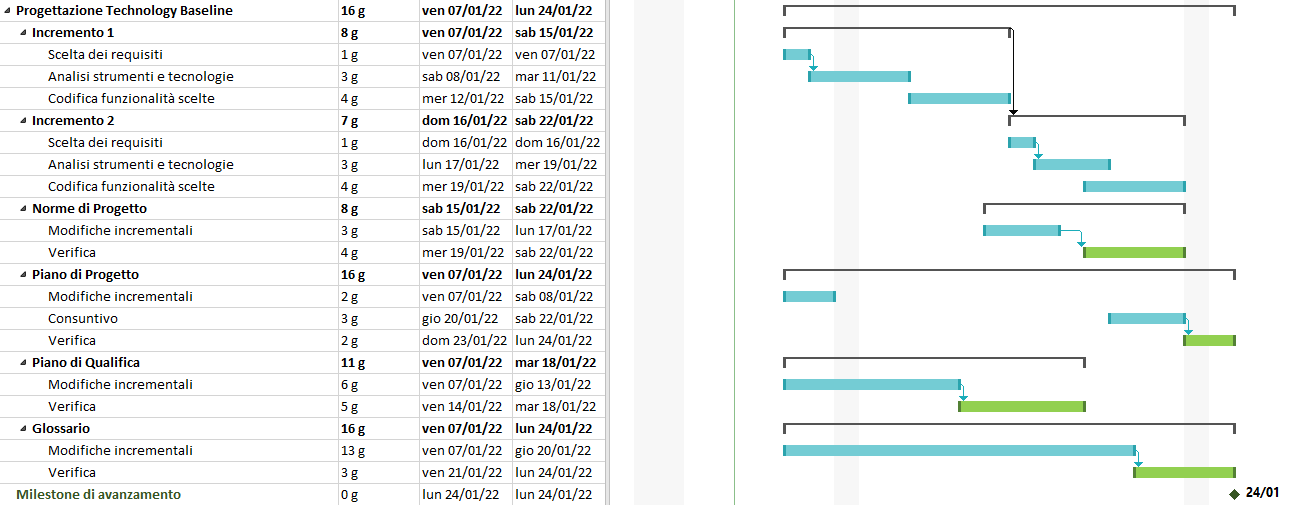
\includegraphics[scale=0.56]{immagini/technology_baseline.png}
  \caption{Diagramma di Gantt - Progettazione Technology Baseline}
\end{figure}
\pagebreak

%%%%%%%%%%%%%%%%%%%%%%%%%%%%%%%%%%%%%%%%%%%%%%%%%%%%%%%%%%%%%%

\subsection{Codifica Proof of Concept} \label{subsection:pianificazione_PoC}
\textbf{Periodo:} dal 2022/01/25 al 2022/02/22.
\bigskip
\\Questo periodo ha inizio dopo il periodo di Progettazione per la Technology Baseline e termina con la scadenza di consegna dei documenti per la revisione di \RTB{} (RTB\glo{}).
In corrispondenza del termine di questo periodo verrà fissato un incontro con il proponente in cui verrà presentato un prototipo del prodotto.
L'attività principale di questo periodo è la realizzazione di un Proof of Concept\glo{}.
Inoltre durante questo periodo vengono effettuati 3 incrementi e 5 modifiche incrementali sui documenti.
\\Le attività svolte sono:
\begin{itemize}
  \item \textbf{Proof of Concept:} Viene realizzato un Proof of Concept\glo{} nel quale devono essere integrate il maggior numero di tecnologie necessarie alla realizzazione del progetto e implementate alcune delle funzionalità principali.
        Il PoC\glo{} è un dimostratore eseguibile e verrà utilizzato come base di partenza su cui poter effettuare incrementi nei periodi successivi.
        L'esito positivo dell'integrazione delle tecnologie implementate nella Technology Baseline garantirà un'alta probabilità di portare a termine il PoC\glo{} con successo;
  \item \textbf{Modifiche incrementali ai documenti:} In questo periodo vengono apportate delle modifiche incrementali sui documenti precedentemente redatti.
\end{itemize}
In questo periodo i ruoli maggiormente coinvolti sono: \roleDesignerLow{}, \roleProgrammerLow{} e \roleVerifierLow{}.
\bigskip
\begin{figure}[H]
  \centering
  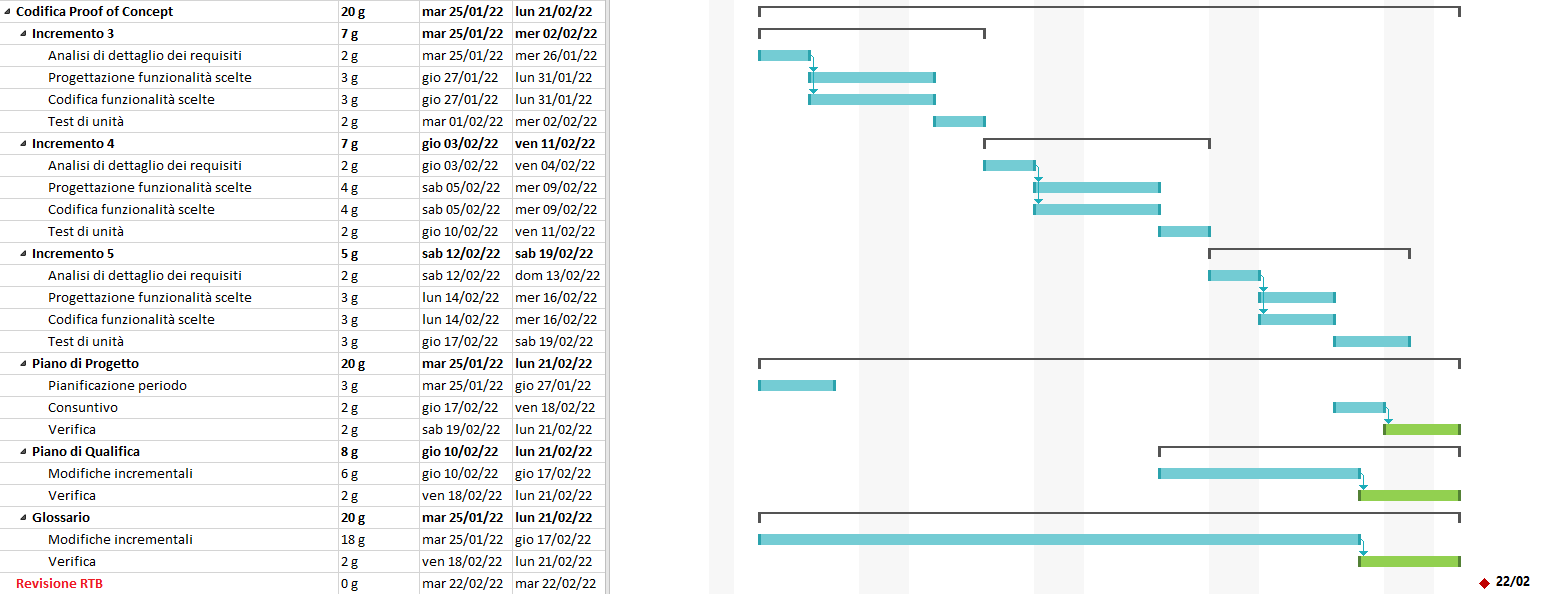
\includegraphics[scale=0.46]{immagini/poc.png}
  \caption{Diagramma di Gantt - Codifica Proof of Concept}
\end{figure}
\pagebreak

%%%%%%%%%%%%%%%%%%%%%%%%%%%%%%%%%%%%%%%%%%%%%%%%%%%%%%%%%%%%%%

\subsection{Progettazione di dettaglio e codifica dei requisiti} \label{subsection:pianificazione_requisiti_obbligatori}
\textbf{Periodo:} dal 2022/03/16 al 2022/05/12.
\bigskip
\\Questo periodo ha inizio dopo la revisione di \RTB{} (RTB\glo{}) e termina con l'inizio del periodo di Validazione e collaudo.
Verrà quindi utilizzato il PoC\glo{} precedentemente creato come base su cui poter incrementare il prodotto.
Una delle attività di questo periodo è la \PB{}, nella quale viene realizzato un allegato tecnico da poter presentare al committente.
Questo periodo, sotto consiglio del committente, abbiamo deciso di dividerlo in Sprint\glo{}, per permettere una riunificazione della produzione documentale a quella software.
Le attività svolte sono:
\begin{itemize}
  \item \textbf{\PB{}:} Questa attività presenta la baseline architetturale del prodotto tramite i diagrammi delle classi e di sequenza, mostrandone la coerenza con quanto mostrato durante l'attività di Technology Baseline.
  \item \textbf{Test:} I \textit{programmatori} scrivono i test di unità e integrazione in relazione ai componenti sviluppati in questo periodo;
  \item \textbf{Codifica:} Viene eseguito lo sviluppo del codice del prodotto da parte dei \textit{programmatori} relativo alle attività selezionate all'inizio dello Sprint\glo{}.
        A partire dalla base creata nel periodo precedente, viene sviluppata una versione funzionante del prodotto tramite aggiunte di funzionalità;
  \item \textbf{Manuali:} Redazione dei documenti \docNameVersionMU{} e \docNameVersionMS{} in relazione alle funzionalità sviluppate.
        Questi documenti forniscono indicazioni sull'utilizzo del sistema da parte degli utenti coinvolti;
  \item \textbf{Modifiche correttive ai documenti:} In questo periodo vengono apportate delle modifiche correttive ai documenti che necessitano di una revisione.
\end{itemize}

\subsubsection{Sprint 1} \label{subsubsection:sprint_1}
\textbf{Periodo:} dal 2022/03/16 al 2022/03/29.
\bigskip
\\Gli obiettivi che il gruppo si prepone per questo sprint\glo{} sono:
\begin{itemize}
  \item Correzione della documentazione in base alle segnalazioni dei committenti;
  \item Preparazione delle attività di progettazione e codifica di dettaglio dei requisiti obbligatori;
  \item Implementazione della funzionalità di pagamento tramite MoneyBox\glo{};
  \item Inizio stesura della documentazione da correlare al prodotto software;
\end{itemize}
Le attività svolte sono:
\begin{itemize}
  \item \textbf{\PB{}:} Inizio stesura dell’allegato tecnico con individuazione dei design pattern;
  \item \textbf{Test:} Vengono scritti i test di unità e integrazione in relazione ai componenti sviluppati in questo periodo;
  \item \textbf{Codifica:} Implementazione della funzionalità di pagamento tramite MoneyBox\glo{};
  \item \textbf{Manuali:} Comincia la redazione dei documenti \docNameVersionMU{} e \docNameVersionMS{} in relazione ai requisiti obbligatori;
  \item \textbf{Modifiche incrementali e correttive ai documenti:} In questo periodo vengono apportate delle modifiche correttive ai documenti che necessitano di una revisione.
\end{itemize}
In questo periodo i ruoli maggiormente coinvolti sono: \roleDesignerLow{}, \roleProgrammerLow{} e \roleVerifierLow{}.
\bigskip
\begin{figure}[H]
  \centering
  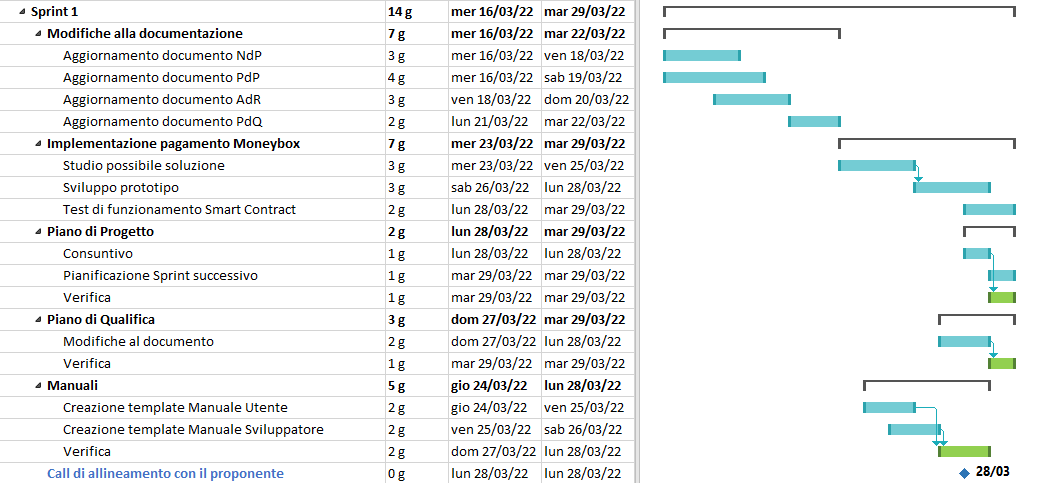
\includegraphics[scale=0.55]{immagini/1sprint.png}
  \caption{Diagramma di Gantt - Sprint 1}
\end{figure}

\subsubsection{Sprint 2} \label{subsubsection:sprint_2}
\textbf{Periodo:} dal 2022/03/30 al 2022/04/12.
\bigskip
\\L'ultimo incontro con il proponente ha sancito la necessità di rivisiatazione della struttura generale, ormai collaudata, per poter realizzare un prodotto facilmente estendibile nel prossimo futuro.
\\Questo cambio di direzione ci porterà a dover ristrutturare elementi già collaudati dell'applicativo.
\\Per questo motivo verranno messi da parte gli obiettivi precedentemente fissati per poter allinearci alle aspettative del proponente.
\\Gli obiettivi che il gruppo si prepone per questo sprint\glo{} sono:
\begin{itemize}
  \item Refactoring dello smart contract\glo{};
  \item Inizio refactoring\glo{} del frontend\glo{} associato;
  \item Continuazione stesura della documentazione da correlare al prodotto software;
\end{itemize}
Le attività svolte sono:
\begin{itemize}
  \item \textbf{\PB{}:} Modifica dell’allegato tecnico con nuova scelta del design pattern da adottare per la nuova soluzione;
  \item \textbf{Test:} Vengono scritti i test di unità e integrazione in relazione ai componenti sviluppati in questo periodo;
  \item \textbf{Codifica:} Viene suddiviso l'unico smart contract\glo{} in due smart contract\glo{} diffenti per le diverse tipologie di pagamento e viene iniziata la riscrittura del frontend\glo{} causata dalle modifiche apportate;
  \item \textbf{Manuali:} Continua la redazione dei documenti \docNameVersionMU{} e \docNameVersionMS{} in relazione ai requisiti selezionati;
  \item \textbf{Modifiche correttive ai documenti:} In questo periodo vengono apportate delle modifiche correttive ai documenti che necessitano di una revisione.
\end{itemize}
In questo periodo i ruoli maggiormente coinvolti sono: \roleDesignerLow{}, \roleProgrammerLow{} e \roleVerifierLow{}.
\begin{figure}[H]
  \centering
  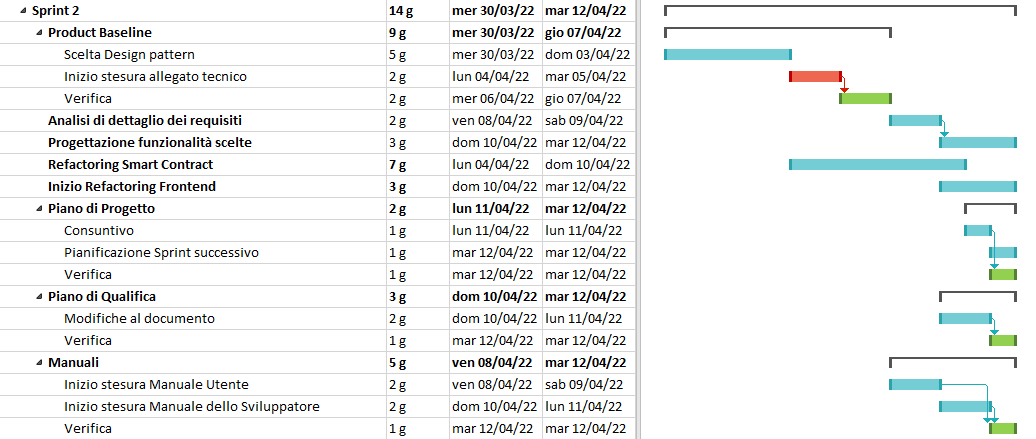
\includegraphics[scale=0.55]{immagini/2sprint.png}
  \caption{Diagramma di Gantt - Sprint 2}
\end{figure}

\subsubsection{Sprint 3} \label{subsubsection:sprint_3}
\textbf{Periodo:} dal 2022/04/13 al 2022/04/22.
\bigskip
\\Gli obiettivi che il gruppo si prepone per questo sprint\glo{} sono:
\begin{itemize}
  \item Preparazione delle attività di progettazione e codifica di dettaglio dei requisiti selezionati;
  \item Continuazione del refactoring\glo{} del frontend\glo{} e riscrittura dei test di unità ed integrazione;
  \item Continuazione stesura della documentazione da correlare al prodotto software;
  \item Incremento della documentazione per la verifica e il miglioramento continuo.
\end{itemize}
Le attività svolte sono:
\begin{itemize}
  \item \textbf{\PB{}:} Continuazione stesura dell’allegato tecnico con implementazione dei diagrammi delle classi;
  \item \textbf{Test:} Vengono riscritti i test di unità ed integrazione in relazione ai componenti modificati in questo periodo;
  \item \textbf{Codifica:} Continuazione del refactoring\glo{} delle componenti frontend\glo{} e scrittura dei test di unità ed integrazione;
  \item \textbf{Manuali:} Continua la redazione dei documenti \docNameVersionMU{} e \docNameVersionMS{} in relazione ai requisiti selezionati;
  \item \textbf{Modifiche correttive ai documenti:} In questo periodo vengono apportate delle modifiche correttive ai documenti che necessitano di una revisione.
\end{itemize}
In questo periodo i ruoli maggiormente coinvolti sono: \roleDesignerLow{}, \roleProgrammerLow{} e \roleVerifierLow{}.
\begin{figure}[H]
  \centering
  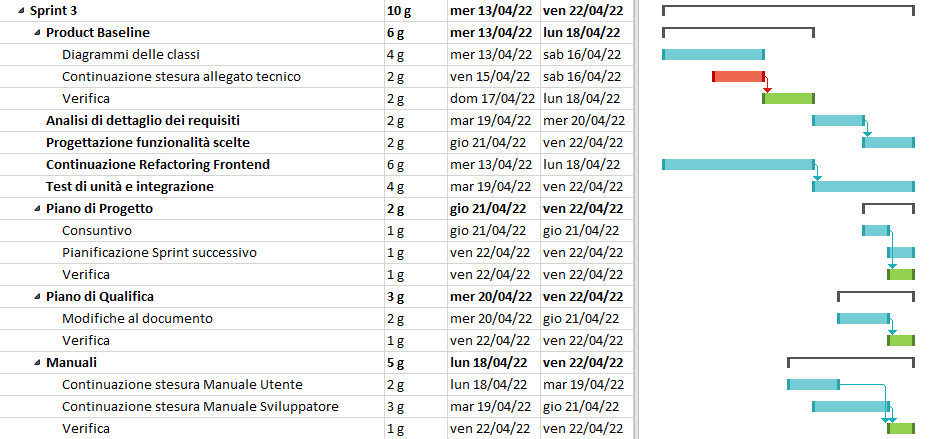
\includegraphics[scale=0.55]{immagini/3sprint.png}
  \caption{Diagramma di Gantt - Sprint 3}
\end{figure}

\subsubsection{Sprint 4} \label{subsubsection:sprint_4}
\textbf{Periodo:} dal 2022/04/23 al 2022/04/29.
\bigskip
\\Gli obiettivi che il gruppo si prepone per questo sprint\glo{} sono:
\begin{itemize}
  \item Continuazione delle attività di progettazione e codifica di dettaglio dei requisiti selezionati;
  \item Aggiunta modalità di pagamento MoneyBox\glo{} con relativo design ed interazione con le altre componenti dell'applicativo;
  \item Continuazione stesura della documentazione da correlare al prodotto software;
  \item Incremento della documentazione per la verifica e il miglioramento continuo.
\end{itemize}
Le attività svolte sono:
\begin{itemize}
  \item \textbf{\PB{}:} Continuazione stesura dell’allegato tecnico con implementazione dei diagrammi di sequenza;
  \item \textbf{Test:} Vengono scritti i test di unità e integrazione in relazione ai componenti sviluppati in questo periodo;
  \item \textbf{Codifica:} Aggiunta la modalità di pagamento MoneyBox\glo{};
  \item \textbf{Manuali:} Continua la redazione dei documenti \docNameVersionMU{} e \docNameVersionMS{} in relazione ai requisiti selezionati;
  \item \textbf{Modifiche correttive ai documenti:} In questo periodo vengono apportate delle modifiche correttive ai documenti che necessitano di una revisione.
\end{itemize}
In questo periodo i ruoli maggiormente coinvolti sono: \roleDesignerLow{}, \roleProgrammerLow{} e \roleVerifierLow{}.
\begin{figure}[H]
  \centering
  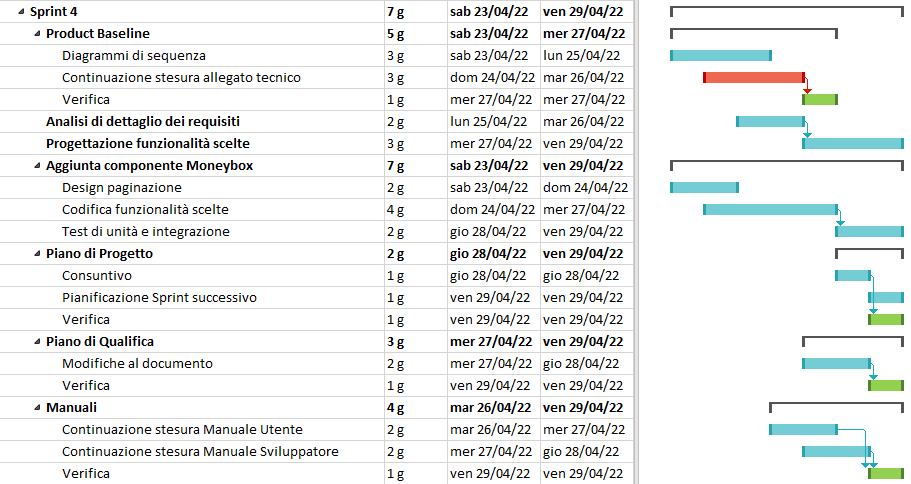
\includegraphics[scale=0.55]{immagini/4sprint.png}
  \caption{Diagramma di Gantt - Sprint 4}
\end{figure}

\subsubsection{Sprint 5} \label{subsubsection:sprint_5}
\textbf{Periodo:} dal 2022/04/30 al 2022/05/06.
\bigskip
\\Gli obiettivi che il gruppo si prepone per questo sprint\glo{} sono:
\begin{itemize}
  \item Continuazione delle attività di progettazione e codifica di dettaglio dei requisiti selezionati;
  \item Abbellimento stile grafico delle pagine;
  \item Continuazione stesura della documentazione da correlare al prodotto software;
  \item Incremento della documentazione per la verifica e il miglioramento continuo.
\end{itemize}
Le attività svolte sono:
\begin{itemize}
  \item \textbf{\PB{}:} Conclusione stesura dell’allegato tecnico;
  \item \textbf{Test:} Vengono scritti i test di unità e integrazione in relazione ai componenti sviluppati in questo periodo;
  \item \textbf{Codifica:} Abbellimento stile grafico delle pagine e fix vari dei bug\glo{} riscontrati;
  \item \textbf{Manuali:} Conclusione stesura \docNameVersionMU{} e continuazione del \docNameVersionMS{} in relazione ai requisiti selezionati;
  \item \textbf{Modifiche correttive ai documenti:} In questo periodo vengono apportate delle modifiche correttive ai documenti che necessitano di una revisione.
\end{itemize}
In questo periodo i ruoli maggiormente coinvolti sono: \roleDesignerLow{}, \roleProgrammerLow{} e \roleVerifierLow{}.
\begin{figure}[H]
  \centering
  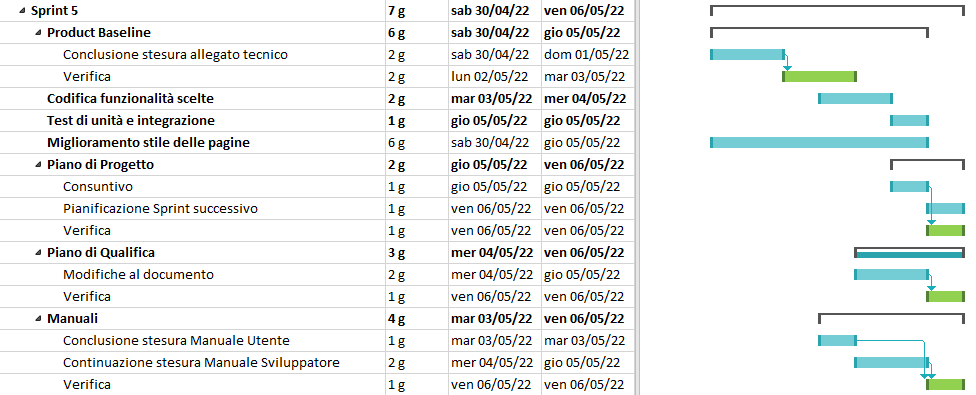
\includegraphics[scale=0.55]{immagini/5sprint.png}
  \caption{Diagramma di Gantt - Sprint 5}
\end{figure}

\subsubsection{Sprint 6} \label{subsubsection:sprint_6}
\textbf{Periodo:} dal 2022/05/07 al 2022/05/12.
\bigskip
\\Gli obiettivi che il gruppo si prepone per questo sprint\glo{} sono:
\begin{itemize}
  \item Continuazione delle attività di progettazione e codifica di dettaglio dei requisiti selezionati;
  \item Sistemazione filtraggio e paginazione delle transazioni effettuate;
  \item Conclusione stesura della documentazione da correlare al prodotto software;
  \item Incremento della documentazione per la verifica e il miglioramento continuo.
\end{itemize}
Le attività svolte sono:
\begin{itemize}
  \item \textbf{Test:} Vengono scritti i test di unità e integrazione in relazione ai componenti sviluppati in questo periodo;
  \item \textbf{Codifica:} Correzioni dei bug\glo{} rimanenti e sistemazione del filtraggio e paginazione delle transazioni effettuate;
  \item \textbf{Manuali:} Conclusione stesura del \docNameVersionMS{};
  \item \textbf{Modifiche correttive ai documenti:} In questo periodo vengono apportate delle modifiche correttive ai documenti che necessitano di una revisione.
\end{itemize}
In questo periodo i ruoli maggiormente coinvolti sono: \roleDesignerLow{}, \roleProgrammerLow{} e \roleVerifierLow{}.
\begin{figure}[H]
  \centering
  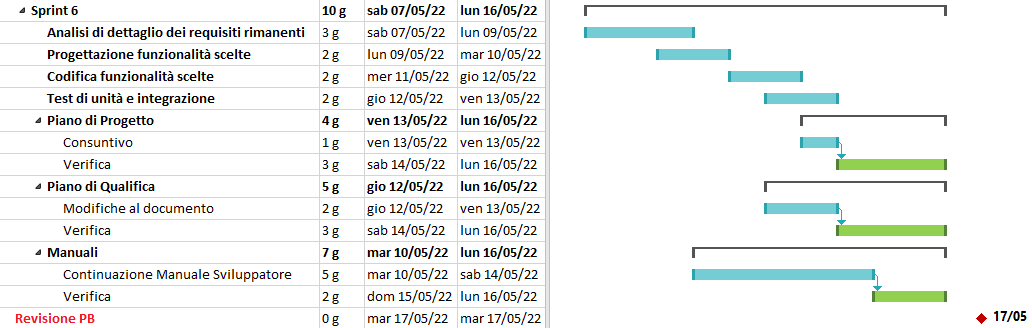
\includegraphics[scale=0.55]{immagini/6sprint.png}
  \caption{Diagramma di Gantt - Sprint 6}
\end{figure}
\pagebreak

%%%%%%%%%%%%%%%%%%%%%%%%%%%%%%%%%%%%%%%%%%%%%%%%%%%%%%%%%%%%%%

\subsection{Validazione e collaudo} \label{subsection:pianificazione_validazione}
\textbf{Periodo:} dal 2022/05/14 al 2022/05/30.
\bigskip
\\Questo periodo ha inizio dopo il periodo di Progettazione di dettaglio e codifica dei requisiti e termina con la scadenza di consegna dei documenti per la revisione di \CA{} (CA\glo{}).
Questo periodo rappresenta l'atto conclusivo delle attività di verifica realizzate precedentemente.
\\Nel primo Sprint\glo{} verranno implementati i requisiti mancanti in attesa della revisione della \PB{} da parte del committente.
Nel secondo Sprint\glo{} il gruppo si concentrerà nella eventuale correzione della documentazione previa revisione e successivamente sarà impegnato nella effettiva validazione e successivo collaudo dell'applicativo.
\\Il sistema verrà collaudato e ci si accerterà che il prodotto realizzato sia pienamente conforme alle aspettative.
Le attività svolte sono:
\begin{itemize}
  \item \textbf{Test:} Vengono eseguiti test di sistema per verificare che il prodotto presenti tutte le caratteristiche attese;
  \item \textbf{Collaudo:} Il prodotto viene eseguito e testato in tutte le sue funzionalità, verificando che siano stati soddisfatti tutti i requisiti;
  \item \textbf{Validazione:} Viene controllato che il prodotto sia conforme alle specifiche e soddisfi le richieste del cliente.
        Durante questa attività vengono eseguiti i test di validazione;
  \item \textbf{Modifiche correttive ai documenti:} In questo periodo vengono apportate delle modifiche correttive ai documenti che necessitano di una revisione.
\end{itemize}
In questo periodo i ruoli maggiormente coinvolti sono: \roleDesignerLow{}, \roleProgrammerLow{} e \roleVerifierLow{}.
\bigskip
\begin{figure}[H]
  \centering
  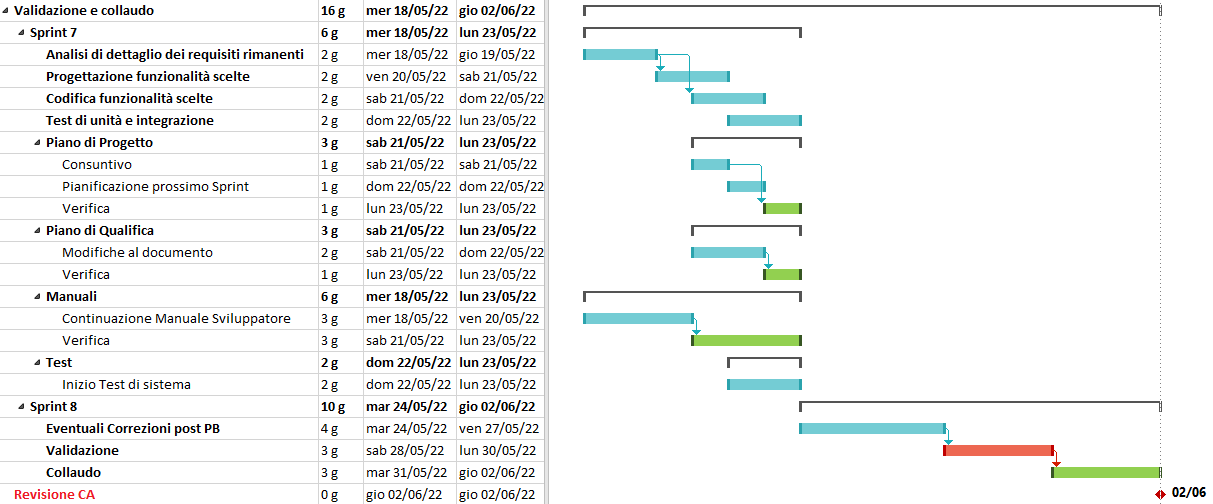
\includegraphics[scale=0.55]{immagini/validazione_collaudo.png}
  \caption{Diagramma di Gantt - Validazione e collaudo}
\end{figure}
\pagebreak